\documentclass{beamer}

% NOTE: reference
% https://arxiv.org/pdf/1604.05488.pdf

% HAGAR, first telescope to operate at an elevation > 4km
% http://www.tifr.res.in/~hagar/
% https://en.wikipedia.org/wiki/Indian_Astronomical_Observatory


\mode<presentation> {\usetheme{Madrid}}

\usepackage{graphicx}
\usepackage[utf8]{inputenc}
\usepackage{amsmath, amsthm, amssymb, mathtools}
\usepackage{hyperref}
\usepackage{flexisym}
\usepackage{mhchem}
\graphicspath{{./img/}}

\title[TeV Astrophysics]{Astronomical facilities and instrumentation in TeV}

\author{Wei-Chih Huang}
\institute[NTHU]{
National Tsing Hua University \\
\medskip
}
\date{April 23, 2019}


\begin{document}

\begin{frame}
	\titlepage % Print the title page as the first slide
\end{frame}

\begin{frame}{Overview}
	\tableofcontents
\end{frame}



%%%% Introduction
%%%%%%%%%%%%%%%%%%%%%%%%%%%%%%%%%%%%%%%%%%%%%%
\section{Introduction to Tev $\gamma$ ray}
\begin{frame}{Introduction to Tev $\gamma$ ray}
	\begin{itemize}
		\item $\gamma$ ray production mechanisms
		\item Astrophysical sources of high-energy $\gamma$ rays
		\item Detection method
		\item Cherenkov radiation
	\end{itemize}
\end{frame}


%%%%%%%%%%%%%%%%%%%%%%%%%%%%%%%%%%%%%%%%%%%%%%%%%%%%%%%%%%%%%
\subsection{$\gamma$ ray production mechanisms}
\begin{frame}{$\gamma$ ray production mechanisms}
	There are several ways to generate cosmic gamma rays:
	\begin{enumerate}
		\item $p_1 + p_2 \rightarrow \gamma + q_1 + ...$
		\item $p^+ + p^- \rightarrow \gamma + \gamma$
		\item $p_0 \rightarrow \gamma + q_1 + ...$
		\item $p \xrightarrow{\text{accelerate}} \gamma + p$
	\end{enumerate}

	Examples:
	\begin{enumerate}
		\item $p_i = proton, nucleus, q = pion \text{ (which decay into a pair of gamma rays)}$
		\item $p^+ = position, p^- = electron$
		\item $p_0 = \text{some heavy nuclei}$
		\item synchrotron radiation $P = \frac{2Ke^2 \gamma^4 v^4}{3c^3r^2} $
	\end{enumerate}
	\setlength{\fboxrule}{0.1pt}{hello}
	\href{https://imagine.gsfc.nasa.gov/science/toolbox/gamma_generation.html}{some animation}
\end{frame}


%%%%%%%%%%%%%%%%%%%%%%%%%%%%%%%%%%%%%%%%%%%%%%%%%%%%%%%%%%%%%
\subsection{Origin of TeV Photons}
\begin{frame}{Origin of TeV Photons}
	leptonic models: inverse Compton scattering

	$\gamma + e^-(e^+) \rightarrow \gamma + e^-(e^+) \Rightarrow \text{photon get energy} $
	\newline
	\newline
	hadronic models: $\pi^0 \ \text{decay}$, synchrotron radiation from ultra-relativistic protons
\end{frame}


%%%%%%%%%%%%%%%%%%%%%%%%%%%%%%%%%%%%%%%%%%%%%%%%%%%%%%%%%%%%%
\subsection{Astrophysical sources of high-energy $\gamma$ rays}
\begin{frame}{Astrophysical sources of high-energy $\gamma$ rays}
	\begin{enumerate}
		\item pulsars
		\item blazars
		\item AGN
		\item pulsar wind nebula
		\item supernova remnant
		\item some particular binary system
		\item the centre of Galaxy
	\end{enumerate}
\end{frame}


%%%%%%%%%%%%%%%%%%%%%%%%%%%%%%%%%%%%%%%%%%%%%%%%%%%%%%%%%%%%%
\subsection{Detection method}
\begin{frame}{Ground-based detector}
	challenges:
	\begin{itemize}
		\item High-energy $\gamma$ ray cannot be focused.
		\item Above 100 MeV, $\gamma$ rays can only be detected by their conversion into $e^+ + e^-$ pairs in matter
		\item electromagnetic cascade
	\end{itemize}

	solutions:
	\begin{itemize}
		\item more sensitive detector
		\item higher altitude experiment
	\end{itemize}
\end{frame}


%%%%%%%%%%%%%%%%%%%%%%%%%%%%%%%%%%%%%%%%%%%%%%%%%%%%%%%%%%%%%
\subsection{Cherenkov radiation}
\begin{frame}{Cherenkov radiation}
	\begin{figure}[h]
		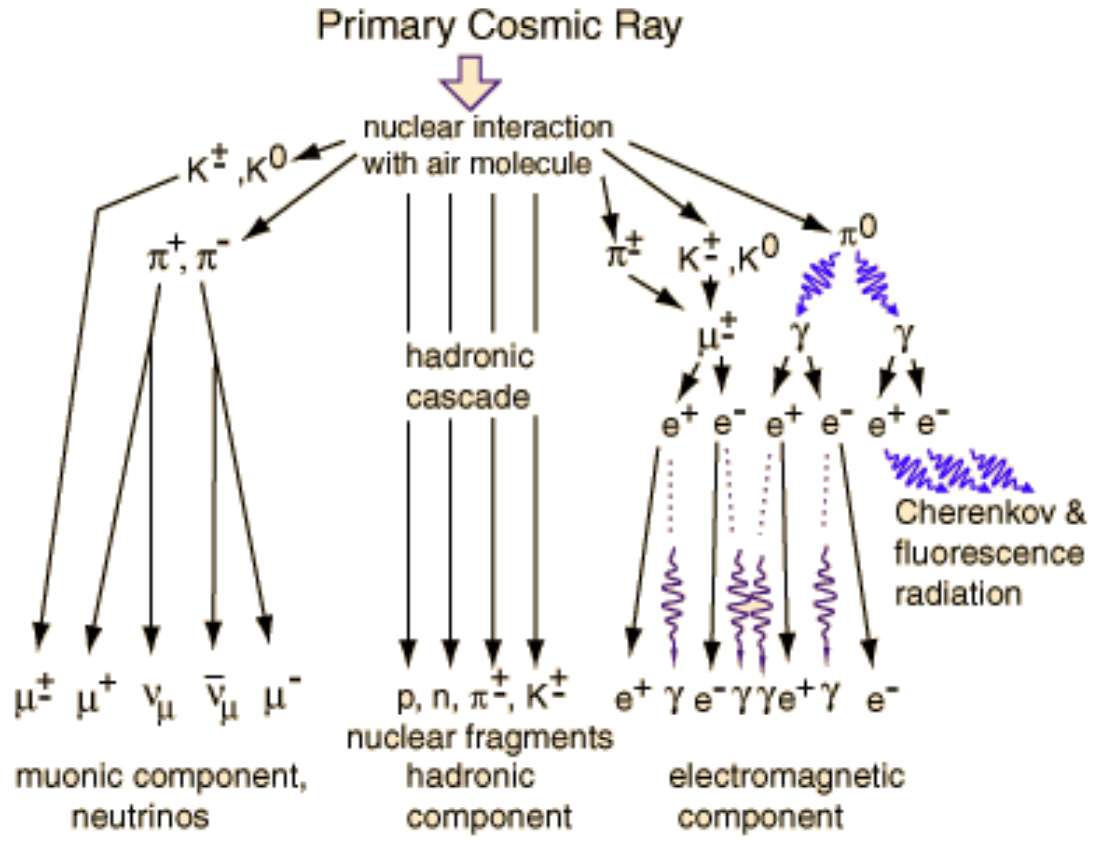
\includegraphics[width=280px]{cara.png}
	\end{figure}
\end{frame}

\begin{frame}{Cherenkov radiation}
	\begin{figure}[h]
		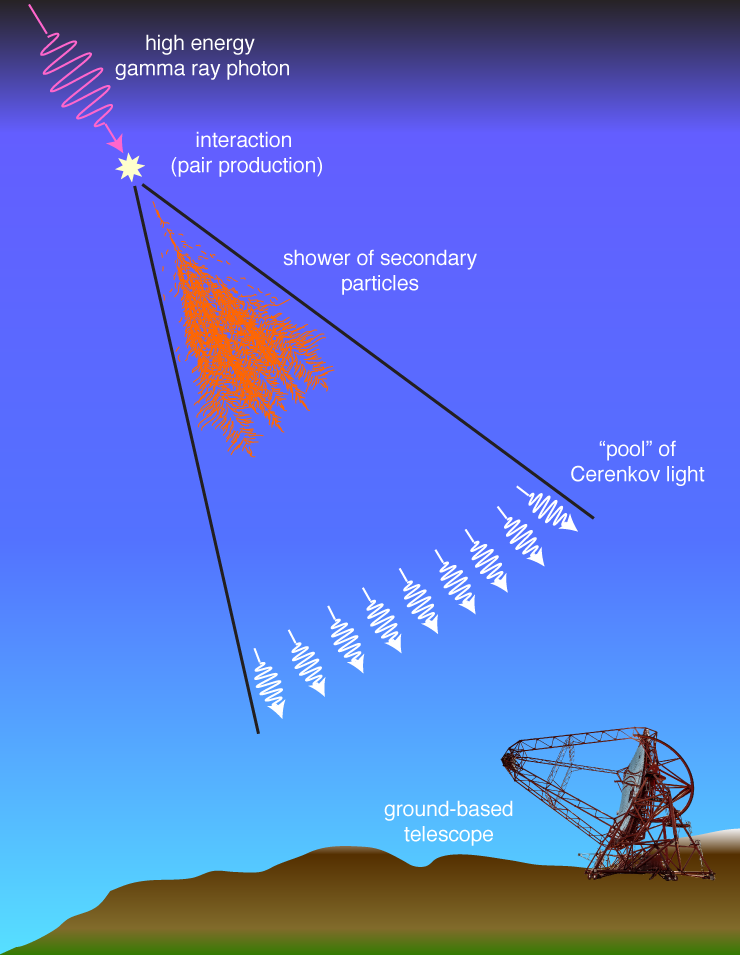
\includegraphics[width=170px]{atmosphere_cerenkov.png}
	\end{figure}
\end{frame}


%%%% Detectors
%%%%%%%%%%%%%%%%%%%%%%%%%%%%%%%%%%%%%%%%%%%%%%%%%%%%%%%%%%%%%
\section{Detectors}
\begin{frame}{Detectors}
	\begin{itemize}
		\item OSO-3 satellite detector
		\item Current ICAT
		\item Future ICAT
	\end{itemize}
\end{frame}



%%%%%%%%%%%%%%%%%%%%%%%%%%%%%%%%%%%%%%%%%%%%%%%%%%%%%%%%%%%%%
\subsection{OSO-3 satellite}
\begin{frame}{OSO-3 satellite}
	OSO 3 (Orbiting Solar Observatory 3)
	\begin{enumerate}
		\item Mar. 8, 1967: launched on
		\item Jun. 28, 1968: tape recorder failed
		\item Nov. 10, 1969: last data were received
		\item Apr. 4, 1982: burned up
	\end{enumerate}
	Result:
	\newline
	The MIT gamma-ray instrument obtained the first identification of high-energy cosmic gamma rays emanating from both galactic and extra-galactic sources
\end{frame}



%%%%%%%%%%%%%%%%%%%%%%%%%%%%%%%%%%%%%%%%%%%%%%%%%%%%%%%%%%%%%
\subsection{Current ICAT}
\begin{frame}{ICAT Properties}
	Properties:
	\begin{enumerate}
		\item 50 GeV $\sim$ 50 TeV in photon energy range
		\item ground-based detector
		\item Wider energy regime than space-based instruments
		\item largest telescope at the highest altitude
		\item work by detecting Cherenkov radiation produced by high energy charged particles
	\end{enumerate}
\end{frame}



\begin{frame}{ICAT components}
	Imaging Atmospheric (or Air) Cherenkov Telescope or Technique
	\newline
	Operating IACT systems:
	\begin{enumerate}
		\item High Energy Stereoscopic System (H.E.S.S.)
		\item Major Atmospheric Gamma Imaging Cherenkov Telescopes (MAGIC)
		\item First G-APD Cherenkov Telescope (FACT)
		\item Very Energetic Radiation Imaging Telescope Array System (VERITAS)
		\item Collaboration of Australia and Nippon for a Gamma Ray Observatory in the Outback (CANGAROO-III)
	\end{enumerate}
	\begin{figure}[h]
		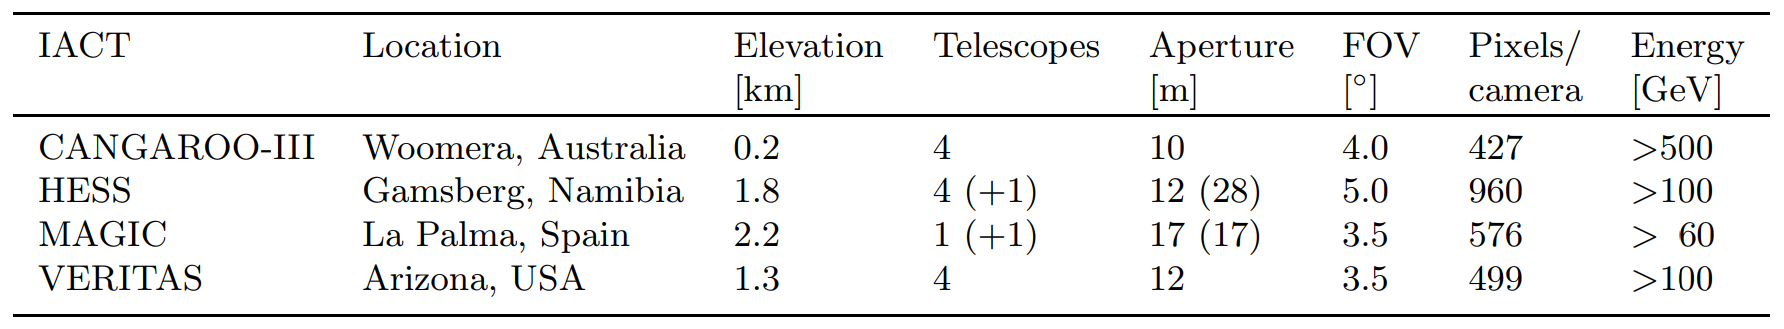
\includegraphics[width=350px]{IACT_tables.png}
	\end{figure}
\end{frame}

\begin{frame}{ICAT components}
	\begin{figure}[h]
		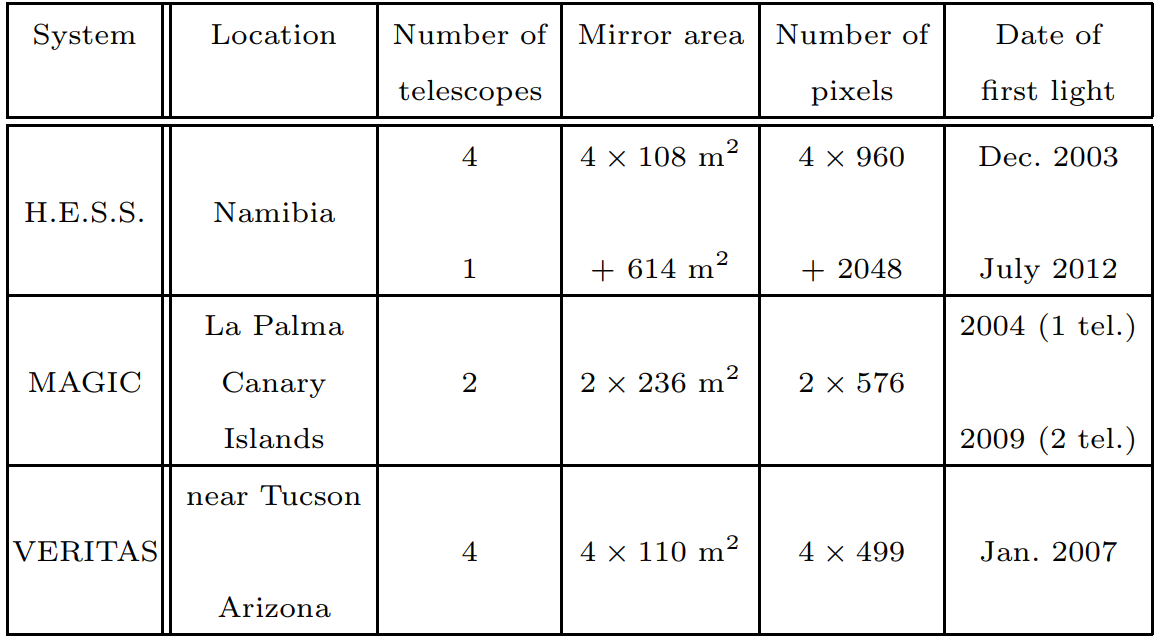
\includegraphics[width=280px]{ICATsystems.png}
	\end{figure}
\end{frame}


\begin{frame}{ICAT components}
	\begin{figure}[h]
		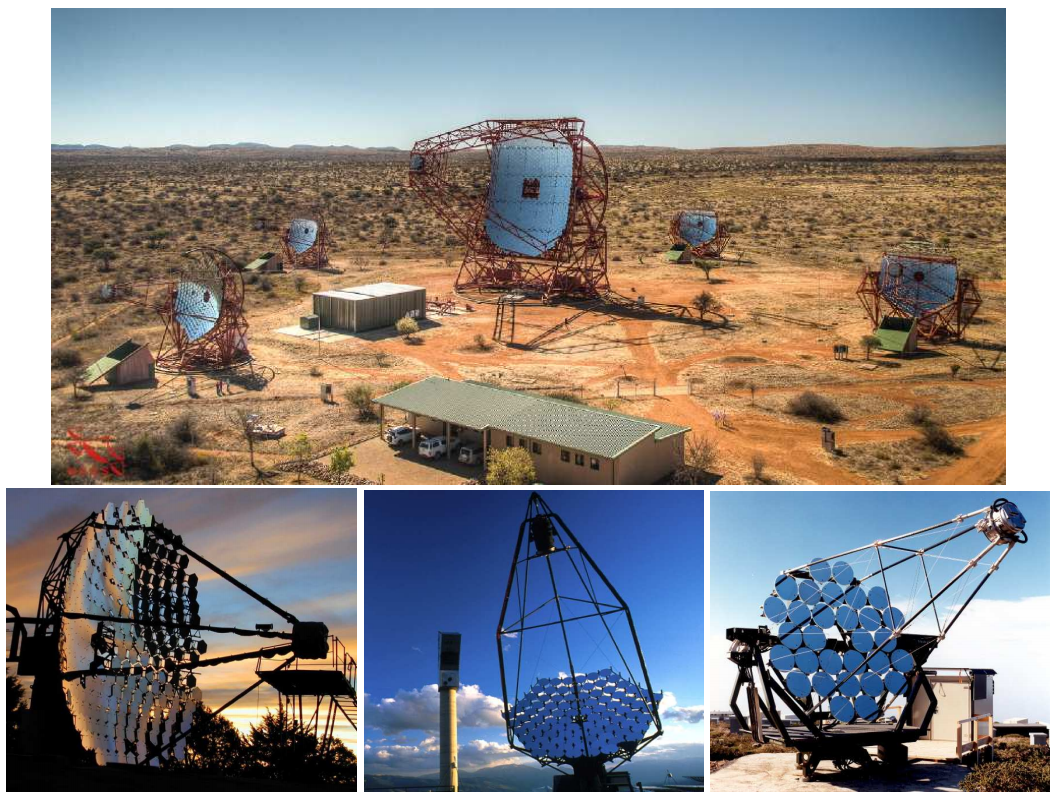
\includegraphics[width=200px]{dishes.png}
		\caption{Illustration of the combination in H.E.S.S. (upper panel) of large dishes as in Whipple (lower left), fast and fine grained cameras as in CAT (lower centre) and stereoscopic observation as in HEGRA (lower right).}
	\end{figure}
\end{frame}


\begin{frame}{ICAT components}
	\begin{figure}[h]
		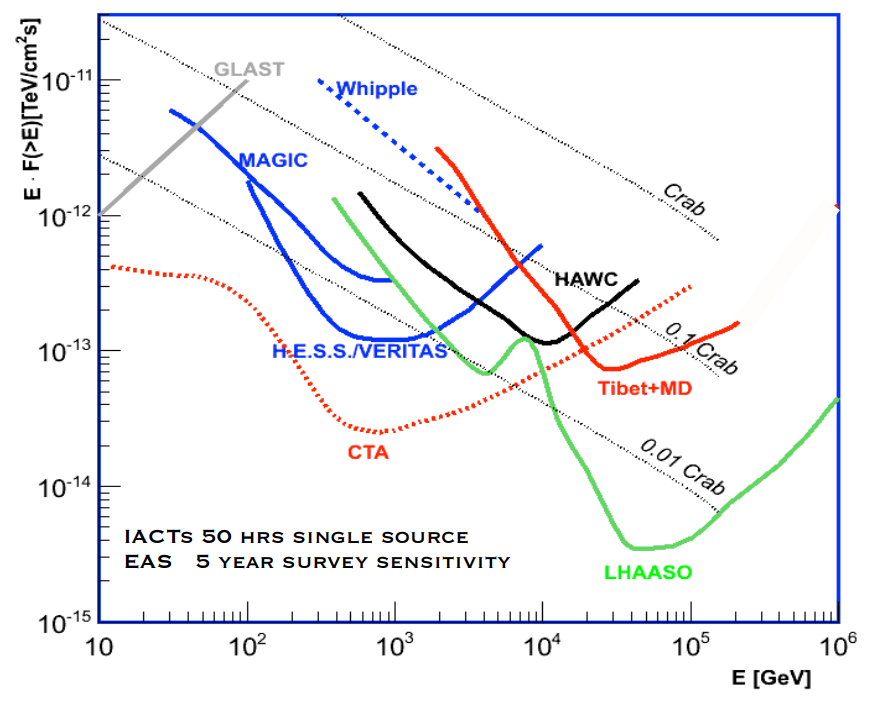
\includegraphics[width=230px]{snesitivities.png}
		\caption{Energy-flux sensitivities of current and future ground-based detectors - the IACT and EAS arrays in the energy range $10^{10}$ to $10^{15}$ eV (courtesy of G. Sinnis).}
	\end{figure}
\end{frame}


%% shown detectors
\begin{frame}{ICAT: FACT}
	G-APD: a new semiconductor device with excellent single photon response became available: the so-called Geiger-mode Avalanche Photodiodes.
	\begin{figure}[h]
		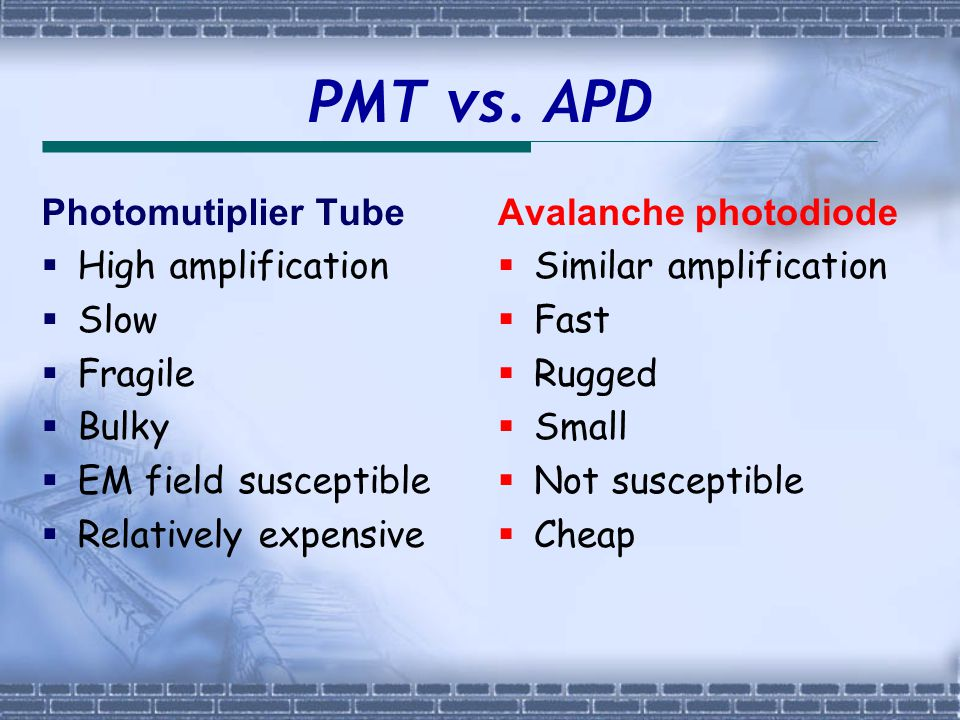
\includegraphics[width=280px]{PMTvsAPD.jpg}
	\end{figure}
\end{frame}


\begin{frame}{ICAT: FACT}
	\begin{figure}[h]
		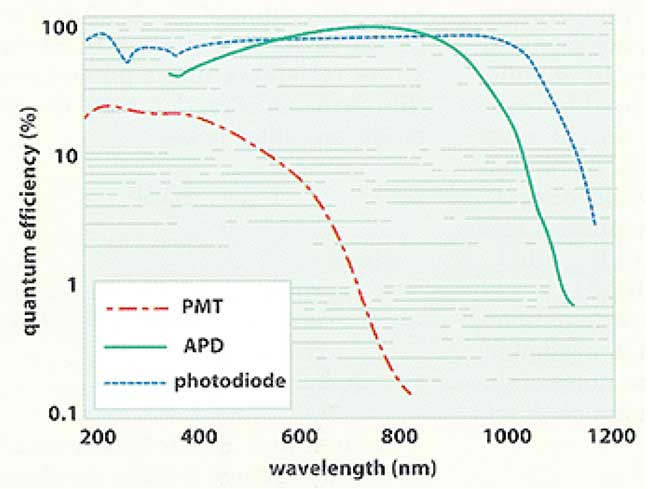
\includegraphics[width=280px]{DetectorsGuidepost.jpg}
	\end{figure}
\end{frame}

% \begin{frame}{ICAT: FACT}
% 	The Photomultiplier (PM) tube
% 	\begin{itemize}
% 		\item Detection of very weak scintillation light
% 		\item Provide electrical signal
% 		\item Can be also done with silicon photodiodes, but PM are most widely used
% 		\item Characterized by spectral sensitivity
% 	\end{itemize}
% \end{frame}


% \begin{frame}{ICAT: FACT}
	% Structure of PM tube
	% \begin{figure}[h]
		% 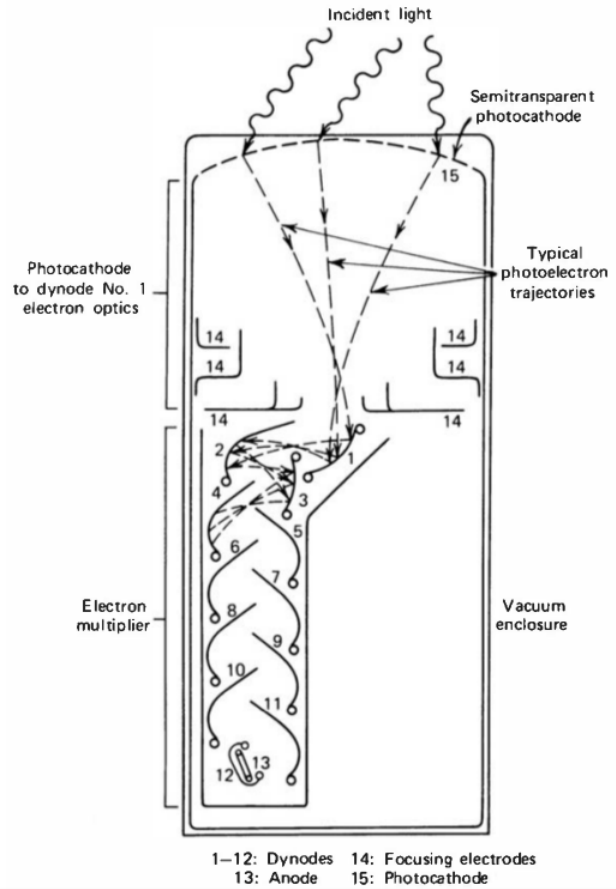
\includegraphics[width=280px]{PM_tube_structure.png}
	% \end{figure}
% \end{frame}


\begin{frame}{ICAT: FACT}
	First G-APD Cherenkov Telescope (FACT), which is based on a former HEGRA telescope.
	\newline
	Upgrade:
	\begin{itemize}
		\item refurbished mirrors
		\item drive system
		\item data acquisition system
	\end{itemize}
\end{frame}


\begin{frame}{ICAT: FACT}
	Mirrors:
	\begin{itemize}
		\item hexagonal shape surface with total area 9.51$m^2$
		\item re-machined by diamond-milling and subsequent coating with \ce{SiO2}.
	\end{itemize}
\end{frame}

\begin{frame}{ICAT: H.E.S.S.}
	High Energy Stereoscopic System (H.E.S.S.)
\end{frame}


\begin{frame}{ICAT: MAGIC}
	Major Atmospheric Gamma Imaging Cherenkov Telescopes (MAGIC)
\end{frame}


\begin{frame}{ICAT: VERITAS}
	Very Energetic Radiation Imaging Telescope Array System (VERITAS)
\end{frame}


\begin{frame}{ICAT: CANGAROO-III}
	CANGAROO-III (Collaboration of Australia and Nippon for a Gamma Ray Observatory in the Outback)
\end{frame}

%%%%%%%%%%%%%%%%%%%%%%%%%%%%%%%%%%%%%%%%%%%%%%%%%%%%%%%%%%%%%
\subsection{Future ICAT}
\begin{frame}{Future ICAT improvement}
	Improvement:
	\begin{enumerate}
		\item enhance flux sensitivities in TeV regime (0.1-10 TeV)
		\item expand energy domain: down to 10 GeV (multi-GeV regime) and well beyond 10 TeV (sub-PeV regime)
	\end{enumerate}
\end{frame}


\begin{frame}{Future ICAT improvement}
	Improvement:b
	\begin{enumerate}
		\item enhance flux sensitivities in TeV regime (0.1-10 TeV)
		\item expand energy domain: down to 10 GeV (multi-GeV regime) and well beyond 10 TeV (sub-PeV regime)

	\end{enumerate}
\end{frame}


\begin{frame}{Future ICAT: TeV regime}
	\begin{enumerate}
		\item minimum detectable energy flux: $10$ erg$/ \text{cm}^2 $ s
		\item angular resolution: $\delta \theta \leq 3$ arc minutes.
	\end{enumerate}
\end{frame}


\begin{frame}{Next generation CTA}
	\begin{figure}[h]
		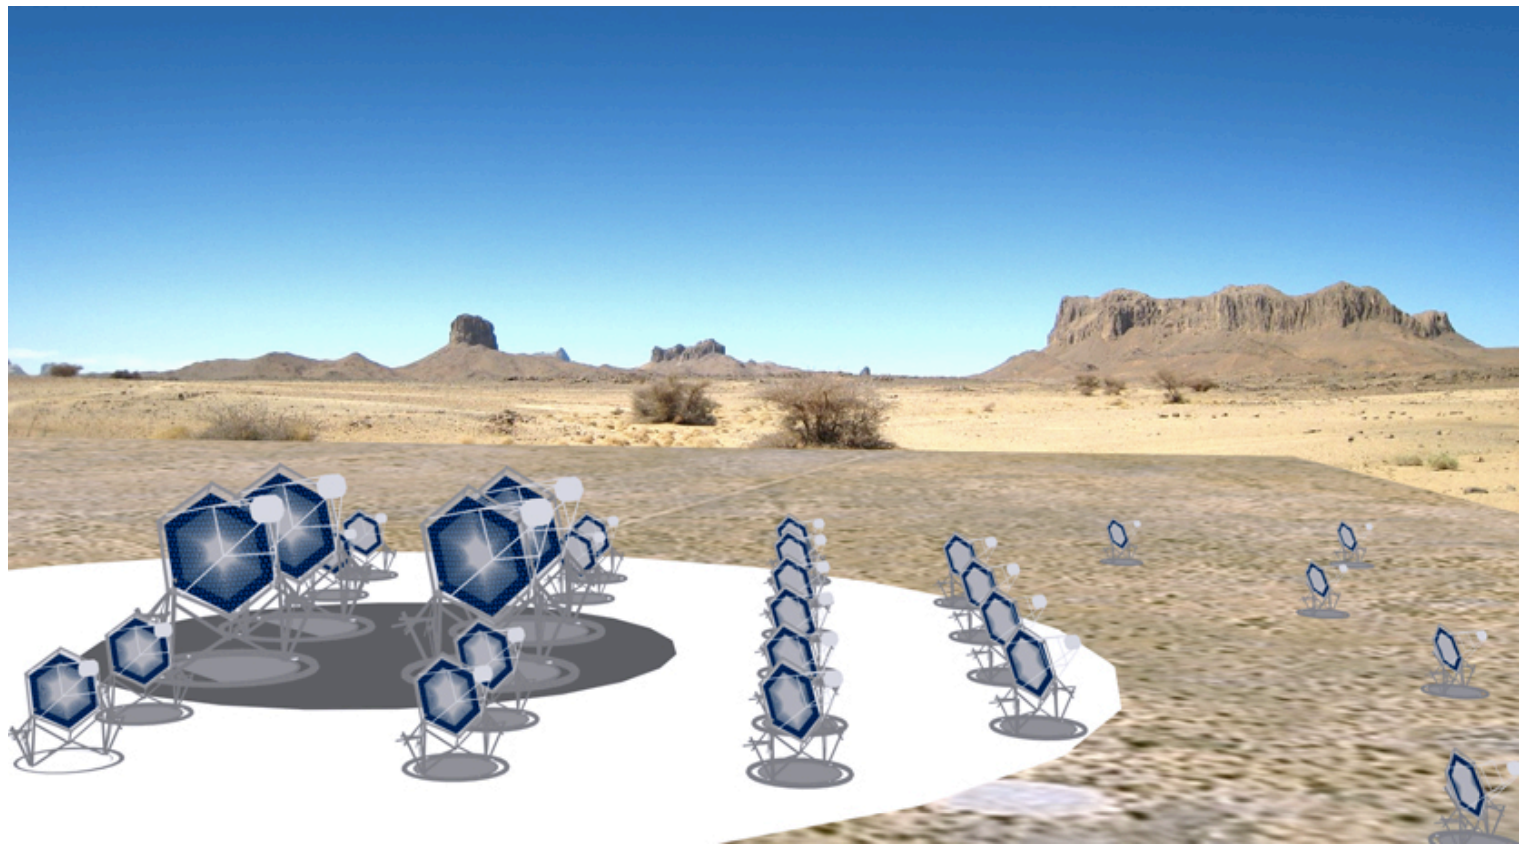
\includegraphics[width=300px]{next-generationCTA.png}
		\caption{Possible layout of the next-generation CTA instrument.
		From Ref}
	\end{figure}
\end{frame}




\end{document}